\documentclass[conference]{IEEEtran}
\usepackage{iftex}
% XeTeX (Tectonic) has no ptm Times; Termes is the same face. pdfLaTeX, e.g. Overleaf, skips this.
\ifXeTeX\usepackage{fontspec}\setmainfont{texgyretermes}[Extension=.otf, UprightFont=*-regular,
  BoldFont=*-bold, ItalicFont=*-italic, BoldItalicFont=*-bolditalic]\fi
\usepackage{cite}
\usepackage{amsmath,amssymb}
\usepackage{graphicx}
\usepackage{booktabs}
\usepackage{url}
\graphicspath{{figures/}}
\hyphenation{Stack-Exchange GARCH}

\begin{document}

\title{What a Small From-Scratch Financial Agent Can Learn from Feedback: Measured Wins, Failures and Traps}

\author{\IEEEauthorblockN{Rishabh Kapur}
\IEEEauthorblockA{Department Name, Institution Name\\
City, Country\\
Email: kapur.rishabh13102003@gmail.com}}

\maketitle

\begin{abstract}
We ask whether an agent can improve its decisions from interaction, outcomes and feedback without
continually retraining its underlying model. We built ALFA, a finance advisory agent, entirely in a
NumPy automatic-differentiation library written for the project, with no external model and no API
keys. It combines a 7.47M-parameter grounded text generator, a volatility head, a retriever and a
tokenised generative model of daily returns. We report every measurement taken, including the
failures. Feedback that moves only a threshold, with the model frozen, halves the gap between
promised and delivered precision (16.7 to 8.5 points after 60 labelled answers). Preference
fine-tuning on community votes did not help: plain DPO raised held-out pair agreement from 58.9\% to
60.9\% while the unsupported-figure rate of free generation rose from 59.4\% to 92.9\%. The cause was
the data: 51.0\% of 62{,}155 question--answer rows state a figure their own retrieved passages do not
contain. Filtering those rows out with the server's own guardrail cut answers containing an invented
figure from 41.0\% to 11.3\% on held-out rows. On prices, direction is not forecastable (35.7\% against a 36.0\% majority class), but the
distribution is. An 876k-parameter return generator beats GARCH(1,1)-t on the one-step log score by
$0.0323 \pm 0.0032$ nats per return over 80{,}576 held-out returns. Its sampled paths reproduce the
tail index and the leverage effect. An online temperature that learns from each realised return,
weights frozen, improves the log score by a further $0.0078 \pm 0.0017$ nats. We also catalogue the
measurement traps that produced false conclusions along the way.
\end{abstract}

\begin{IEEEkeywords}
Learning from feedback, grounded generation, preference optimisation, faithfulness, volatility
forecasting, GARCH, generative models, proper scoring rules, abstention.
\end{IEEEkeywords}

\section{Introduction}
Most published stock-prediction systems report accuracy on a single target, often with little
control for leakage~\cite{Eapen_2019,Lee_2019,Barra_2020}. Most feedback-learning systems retrain a
large pretrained model~\cite{Lin_2020,Wong_2024,rafailov2023dpo}. We studied a harder and smaller
setting. The agent is built from scratch on one CPU. It may not call an external language model. It
must answer conversational finance questions without inventing figures. Its research question is
whether it can get better from interaction, outcomes and feedback \emph{without} continually
retraining its underlying model.

The system separates four concerns. \emph{Knowledge} is a frozen encoder plus retrieved documents.
\emph{Reasoning} is code. \emph{Policy} is the only part that learns. \emph{Memory} is per user.
Policy learning can therefore live in a threshold, a calibrator, a sampling temperature or a reward,
as well as in weights. We measured each.

Our contributions are:
\begin{enumerate}
\item A complete from-scratch system and its evaluation discipline: date-based splits, one margin
rule for every promotion, generate-and-check before loss, and point-in-time serving pinned by tests.
\item Evidence that feedback moving only a policy parameter measurably improves the agent, with the
model frozen (Sections~\ref{sec:policy} and~\ref{sec:online}).
\item A negative result on preference learning, traced to its cause: an unfaithful corpus, which a
rule-based verifier measures directly (Section~\ref{sec:preference}).
\item A tokenised generative return model that beats GARCH-t on the log score and reproduces stylized
facts GARCH cannot, and a precise account of where it does not win (Section~\ref{sec:returns}).
\item A catalogue of the measurement traps we hit, each of which produced a false conclusion
before it was caught (Section~\ref{sec:traps}).
\end{enumerate}

\section{Related Work}
\textbf{Deep learning for stock prediction.} CNN--BiLSTM index predictors~\cite{Eapen_2019},
reinforcement learning on chart images~\cite{Lee_2019} and time-series-to-image
encoders~\cite{Barra_2020} report directional gains. A recent IEEE review~\cite{Li_2024} surveys the
architectures. Large 2026 benchmarks are sceptical. Time-series foundation models forecasting hourly
returns for 1{,}000 US equities collapse to near-flat predictions~\cite{collapse2026}. Across 43
models, generic accuracy ``does not necessarily translate into useful financial
forecasts''~\cite{finverse2026}.

\textbf{Volatility and distributions.} GARCH~\cite{Bollerslev_1986} with Student-t
innovations~\cite{Bollerslev_1987} remains the reference. Neural alternatives are older than deep
learning~\cite{Refenes_2001} and continue in hybrid forms~\cite{Liao_2020}. Chronos~\cite{ansari2024chronos}
showed that a plain language model learns time series once values are scaled and quantised into
tokens.

\textbf{Synthetic financial series.} GANs generate synthetic series in smart
grids~\cite{Zhang_2018} and finance~\cite{Wang_2025}. Quant GANs~\cite{Wiese_2020} evaluate against
the stylized facts of Cont~\cite{Cont_2001} and report training that does not converge. We use their
metrics and a likelihood objective that does converge.

\textbf{Learning from feedback.} Interactive reinforcement learning from human
feedback~\cite{Lin_2020} and RLHF for code~\cite{Wong_2024} learn from judgements, and RLHF has known
vulnerabilities~\cite{McIntosh_2024}. DPO~\cite{rafailov2023dpo} removes the reward model. Adding the
chosen answer's likelihood~\cite{pang2024rpo} anchors it. DeepSeekMath~\cite{shao2024deepseekmath}
writes SFT, DPO, PPO and GRPO as one gradient that differs only in data source, reward and weighting.
Verifiable rewards~\cite{lambert2024tulu}, reward-ranked fine-tuning (RAFT)~\cite{dong2023raft},
self-taught filtering~\cite{zelikman2022star} and dynamic sampling~\cite{yu2025dapo} replace the
learned judge with a check. Continual fine-tuning forgets~\cite{Luo_2025}, which motivates learning
outside the weights.

\textbf{Faithful retrieval-augmented generation.} RAG~\cite{lewis2020rag} grounds answers in
retrieved text, and BM25~\cite{Robertson_2009} remains a strong retriever. Rewarding correct answers
does not buy faithful citations~\cite{postrational2026}. A faithfulness-only reward is won by terse
replies, so financial RAG needs an informativeness term~\cite{yin2026rlfkv}.

\textbf{Scoring.} Strictly proper scoring rules~\cite{Gneiting_2007} reward only honest distributions.
Prequential evaluation~\cite{Dawid_1984} scores each forecast before its outcome is learned from.
Paired comparisons follow Diebold and Mariano~\cite{Diebold_1995}. Tail indices use Hill's
estimator~\cite{Hill_1975}.

\section{System and Data}
\label{sec:system}
\subsection{Constraints}
The constraints are fixed. There is no external model and no API key. Deep-learning frameworks are
banned by an import test, so every model is built on the project's own NumPy code: 445 lines of
autograd and 928 with the layers and optimiser, checked against finite differences. There is no look-ahead: every split is by date, and every served
figure is rebuilt from bars up to its as-of date, pinned by tests that mutate the data after that
date. No real money is traded. Everything runs on one laptop CPU.

\subsection{Data}
The collector fetches only public bulk endpoints, official APIs and RSS feeds. It honours
\texttt{robots.txt}, allows one request at a time per host, and records the URL and licence of each
file in a manifest of 177{,}358 entries (8.1\,GB). The collection comprises:
\begin{itemize}
\item \textbf{Prices:} daily OHLCV for 101 US and Indian equities. Histories start between 1962 and
2017 and end on 18~September 2026.
\item \textbf{Question--answer pairs:} Stack Exchange (\emph{money}, \emph{economics},
\emph{quant}), giving 62{,}155 supervised pairs and 24{,}639 vote-ranked preference triples.
\item \textbf{Pretraining text:} 798{,}784 sequences of 128 tokens, about 102M tokens, under an
8{,}000-piece WordPiece vocabulary.
\item \textbf{News:} 1{,}481 deduplicated articles from 55 feeds.
\end{itemize}

\subsection{Models}
Fig.~\ref{fig:arch} shows the agent. A 4-layer, 256-wide encoder was pretrained by masked language
modelling. The run took 49{,}232 steps and 11.09\,h, reaching a validation perplexity of 20.6. The
grounded generator (7{,}472{,}192 parameters) adds a 2-layer decoder that cross-attends to four
retrieved 128-token passages, fused in the decoder. A guardrail extracts every figure in an answer
and refuses the turn if any figure is absent from the evidence. The price head is a 202{,}755-parameter
GRU over 128-bar windows. The return generator is described in Section~\ref{sec:returns}.

\begin{figure*}[t]
\centering
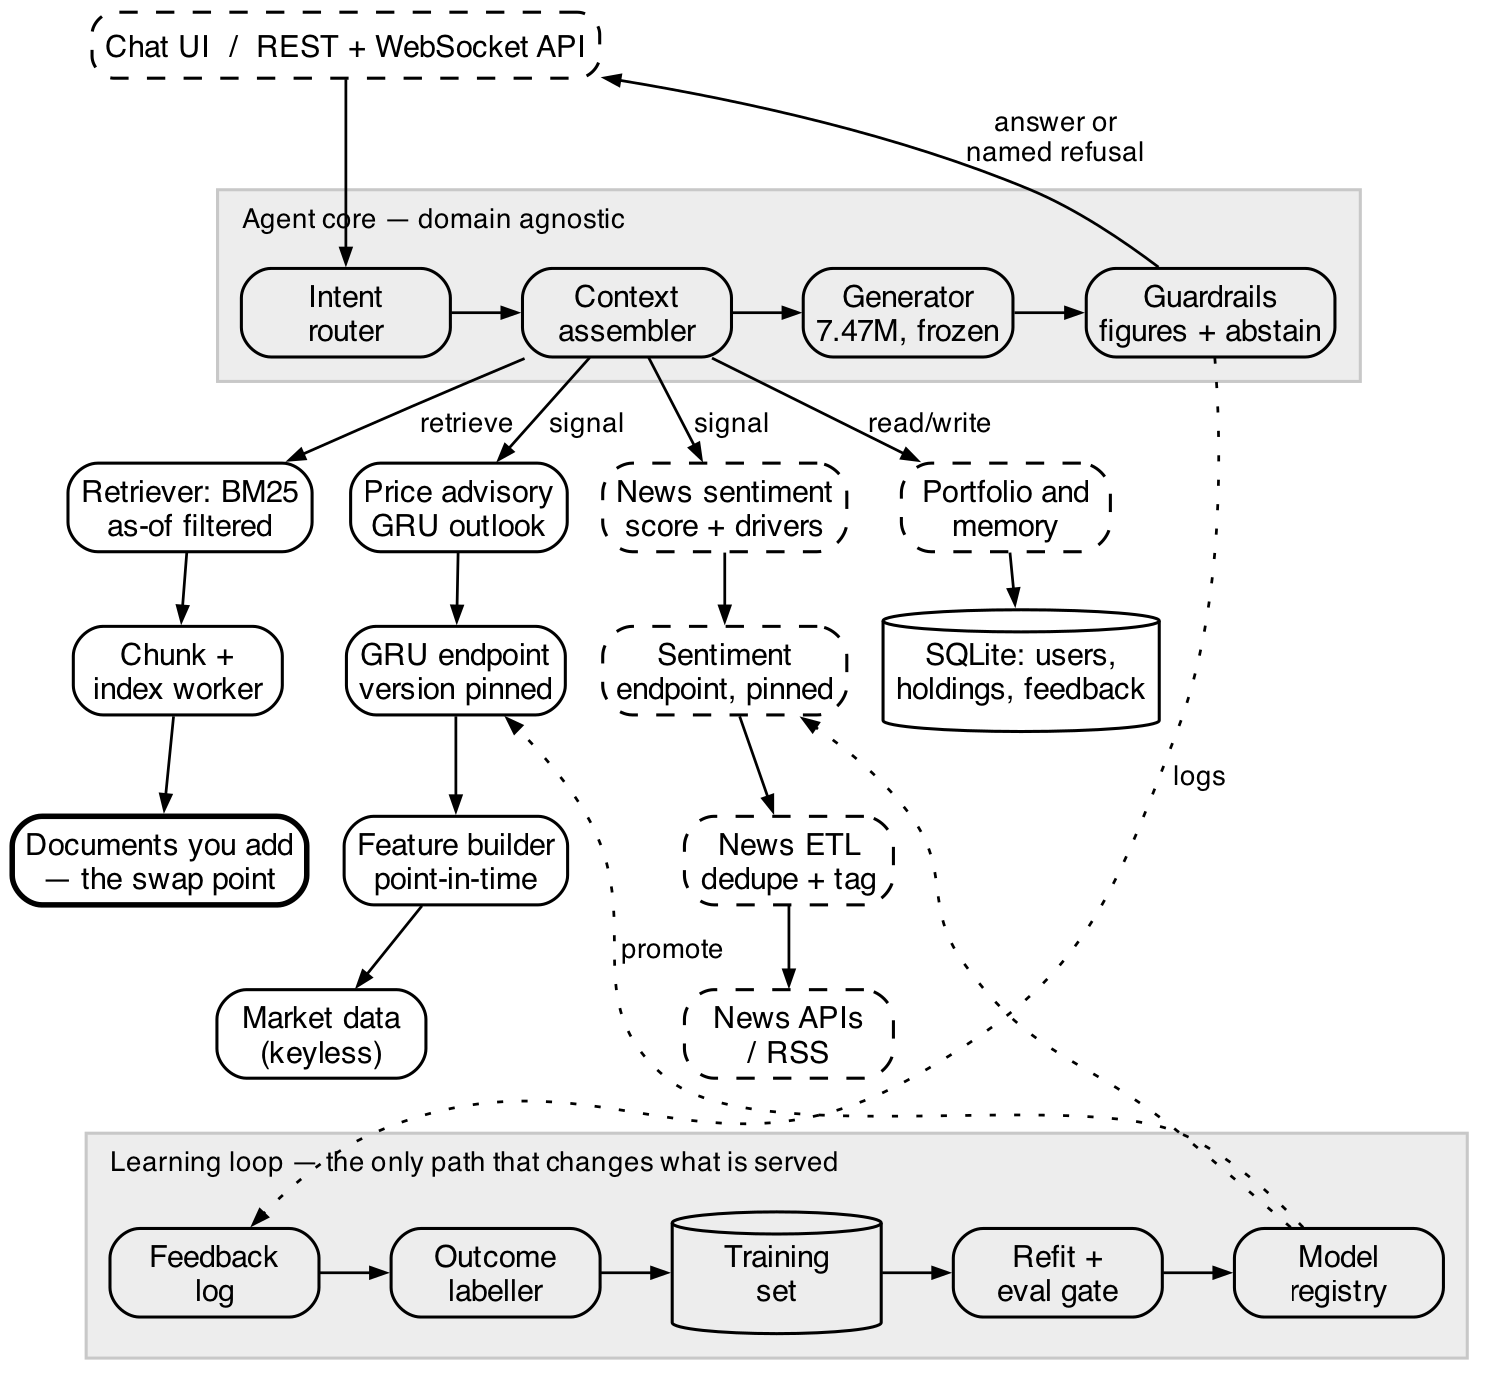
\includegraphics[width=0.62\textwidth]{architecture.png}
\caption{ALFA. The agent core (top) routes a question, assembles evidence, generates with frozen
weights and screens the answer. The learning loop (bottom) is the only path that changes what is
served, and every change passes an evaluation gate.}
\label{fig:arch}
\end{figure*}

\subsection{Evaluation discipline}
Three rules apply throughout:
\begin{enumerate}
\item \textbf{One margin rule.} A candidate replaces what is served only if it beats it by more than
one standard error of the difference, measured on identical rows.
\item \textbf{Generate, then check.} A text model is judged by answers it writes, not by loss.
\item \textbf{Held-out means untouched.} Every quoted figure comes from a period, phrasing or split
that chose nothing.
\end{enumerate}
The S14 faithfulness standard requires unsupported figures below 2\%.

\section{Grounded Generation}
\label{sec:grounded}
\subsection{Copying is a late phase transition}
On a synthetic advisory set of 225{,}309 rows, generated from computed indicators, training loss sat
at 0.28 through step 3{,}000 and then collapsed to 0.014 by step 5{,}400. At step 3{,}000,
generate-and-check found 0\% exact match and an unsupported figure in every answer. At step 4{,}000 it
found 45.8\% exact match and 10.5\% unsupported figures. The 0.28 plateau is the entropy of each
field's marginal prior: the model emits the distribution of \emph{close}, not this row's close. It
is not a capacity floor.

\subsection{The decoder reads its evidence}
On the converged model, hiding the evidence costs $+1.042$ nats and swapping in another row's evidence
costs $+1.946$. The swap costing more than the blank shows that the model reads what it is given. On
the real Stack Exchange task, by contrast, hiding every passage costs only $+0.018$. Only 30.7\% of an
answer's content words appear anywhere in its input, so ignoring the evidence is the loss-minimising
strategy there.

\subsection{Sentence shape, not vocabulary}
Unseen phrasings stalled at a loss of 0.70 while trained phrasings reached 0.011. A probe over 190
composed phrasings located the cause. The pretrained encoder places an unseen \emph{word} correctly
in 100\% of cases, but an unseen \emph{frame} in only 68\%. Task fine-tuning halves the latter to
32\%, which is forgetting~\cite{Luo_2025} measured directly. Two fixes followed. Rebuilding the data
from 46 to 190 phrasings cut the unseen floor to 0.2821. Freezing the encoder then cut it to 0.1717,
and unsupported figures on unseen phrasings from 4.7\% to 0.7\%. The promoted checkpoint states
4 of 771 figures (0.5\%) unsupported on reworded questions, with 36.0\% exact match.

\subsection{Decoding}
Greedy decoding repeated 73\% of its 4-grams, against 1.7\% for human answers. Nucleus sampling at
temperature 0.9 and top-$p$ 0.9 measures 1.6\% repeats and 0.4\% invented words.

\section{Learning With the Model Frozen}
\label{sec:policy}
\subsection{Calibration and abstention}
The raw confidence claims 0.99 on answers that are right 31\% of the time. A two-parameter Platt fit
lowers the calibration error from 0.683 to 0.121 over 25 splits. Its ranking AUC is $0.740 \pm 0.039$,
which caps any threshold or reranker built on it. The agent is then given a precision promise
(``answer only when at least $p$ likely to be right'') and solves for the confidence cut from the
feedback it has.

Fig.~\ref{fig:curve} scores the \emph{miss}: the gap between promised and delivered precision, on rows
the cut was not fitted on. At a 60\% bar, 60 feedback rows cut the miss from 16.7 points (the
hand-picked cut) to 8.5. Answering everything misses by 29.2. At an 80\% bar under the agent's labels,
the miss falls monotonically from 13.3 to 6.3 and is still falling at 118 rows. No weight changed.

\begin{figure}[t]
\centering
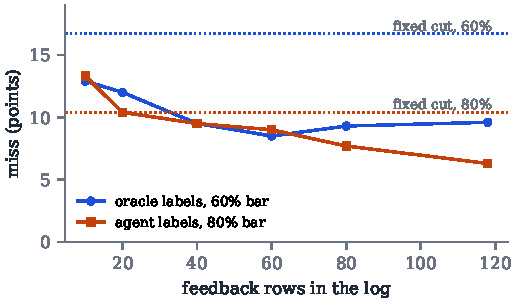
\includegraphics[width=\columnwidth]{learning_curve.pdf}
\caption{Feedback moves only the abstention threshold, and the delivered precision approaches the
promised one. Dotted lines: the hand-picked cut with no feedback.}
\label{fig:curve}
\end{figure}

In a 20-turn session over a live WebSocket, the fitted cut moved from 0.998 to 0.971 at the tenth
judged turn. It \emph{loosened}, because the log did not justify withholding anything. The agent spoke
on 14 of 17 judged turns and was right on 13 of them (92.9\%).

\subsection{Routing with frozen weights}
Summing the frozen encoder's cosine with the share of the question's term weight that known
phrasings cover raises routing accuracy on an unseen sentence shape from 67\% to 90\%. Rewriting a
question into its routed trained phrasing raises held-out exact match from 33.5\% to 74.5\%. Twelve of
twelve out-of-domain questions are refused. No parameter was fitted.

\subsection{Best-of-$k$ does not pay}
Eight samples from the advisory generator contain 1.77 distinct answers. Best-of-8 by confidence
scores 27.8\% and by grounding tier 28.5\%, against 28.0\% for a single sample on 600 rows. A model
whose token distribution is nearly a delta cannot be improved by sampling it more.

\section{Preference Learning, and Why It Failed}
\label{sec:preference}
\subsection{How good are the labels?}
A blind reader judged 60 held-out vote-ranked pairs with the sides shuffled, and agreed with the votes
on 40 (66.7\%, roughly $\pm 6$ points). A third of the training labels are judgements a careful reader
would not make. The reader was the AI assistant used in development, not a domain expert.

\subsection{Plain DPO collapses}
One epoch of DPO ($\beta = 0.1$, length-normalised, reference fixed) on 22{,}379 pairs lowered the
held-out loss from 0.6931 to 0.6617. Agreement rose from 58.9\% to 60.9\%, but McNemar's test on the
flips (419 right, 379 wrong) gives $p = 0.17$. Free generation collapsed (Table~\ref{tab:dpo}): every
answer opened with about thirty copies of ``you''. The mechanism is measurable. Among 5{,}226 frequent
tokens, ``you'' has the 4th-highest over-representation in preferred answers (1.929\% against
1.867\%). Raising one frequent unigram raises the mean log-probability of the chosen side slightly
more than the rejected side on nearly every pair, which wins the objective without reading either
answer. Loss and agreement improved throughout, and neither could see the failure.

\begin{table}[t]
\centering
\caption{Preference training on vote labels (held out)}
\label{tab:dpo}
\begin{tabular}{@{}lccc@{}}
\toprule
 & Frozen & DPO & DPO + NLL \\
\midrule
Pair agreement (2{,}000) & 58.9\% & 60.9\% & 59.2\% \\
Repeated 4-grams & 1.7\% & 30.8\% & 0.3\% \\
Unsupported figures & 59.4\% & 92.9\% & 74.3\% \\
Answers with an invented figure & 39.0\% & 59.0\% & 40.0\% \\
\bottomrule
\end{tabular}
\end{table}

Adding the chosen answer's negative log-likelihood~\cite{pang2024rpo} fixed the collapse (0.3\%
repeats) but learned nothing. At the default weight of 1.0 the supervised gradient is about 20 times
the ranking gradient, whose magnitude is bounded by $\beta$. Neither run beat the frozen checkpoint,
and nothing was promoted.

\subsection{The root cause is the corpus}
Among 4{,}000 sampled supervised rows, 2{,}390 state at least one figure, and only 116 of those
(4.9\%) have every figure in their retrieved passages. On the full build, 31{,}719 of 62{,}155 rows
(51.0\%) state a figure their passages do not contain. The generator's unsupported-figure rate is
this data learned correctly. Both sides of a preference pair are drawn from the same corpus, so no
ordering between them expresses grounding.

\subsection{From labels to a check}
Following the verifiable-reward literature~\cite{lambert2024tulu,dong2023raft}, the reward is the
guardrail itself. An answer that states an unsupported figure scores 0. A refusal scores 0.1. A
grounded answer scores $1 + 0.5 \times$ its number of grounded figures, so going quiet cannot win, as
RLFKV warns~\cite{yin2026rlfkv}. Groups in which every sample scores the same are dropped, following
DAPO~\cite{yu2025dapo}. A dry run on 96 questions with 8 samples each found 87 teachable groups, 9 with
identical scores, none in which every sample invented a figure, and 8.00 distinct answers out of 8.
The loop therefore has signal on that model. Run from the grounded generator described next, it did
not pay. The grounded model states few figures, so 129--132 of 192 groups a round scored alike and
only about 8 training steps a round remained. The first round read 65.6\% to 54.9\% unsupported on
its 200 selection answers. On 300 independent rows it scored 63.0\% against the frozen model's
53.8\%, with 44 supported figures against 61. That was selection noise, and the two later rounds were
refused by a guard against winning the rate by saying less.

\subsection{Filtering the corpus with the same check}
The same rule, applied to the training targets, keeps 30{,}436 of the 62{,}155 rows. A generator
retrained on them was compared with the original on 300 held-out rows that neither saw in
training. The two splits were drawn independently, and 949 of the original 2{,}000 validation rows
had landed in the filtered training set, so those were removed first. The remaining rows lean
towards questions whose passages lack the figures, which is why the original model scores worse on
them than on the full split. Table~\ref{tab:grounded} gives the result. Unsupported figures fell
from 89.0\% to 53.8\%, and answers containing an invented figure from 41.0\% to 11.3\%. The drop
is not the model going quiet: it states more supported figures than before, 61 against 52. The
prose is still incoherent in both models, so faithfulness improved and fluency did not.

\begin{table}[t]
\centering
\caption{Generator retrained on the filtered corpus (300 clean held-out rows)}
\label{tab:grounded}
\begin{tabular}{@{}lcc@{}}
\toprule
 & Original & Filtered corpus \\
\midrule
Figures stated & 474 & 132 \\
Unsupported figures & 422 (89.0\%) & 71 (53.8\%) \\
Supported figures & 52 & 61 \\
Answers with an invented figure & 41.0\% & 11.3\% \\
Repeated 4-grams & 0.9\% & 0.7\% \\
\bottomrule
\end{tabular}
\end{table}

\section{Prices: Direction, Volatility, Retrieval, News}
\label{sec:prices}
Table~\ref{tab:price} summarises the results. Five-day \textbf{direction} is not learnable: the
transformer scored 35.7\% and the GRU 33.5\%, against 36.0\% for the majority class, with the loss
flat at $\ln 3$. Five-day \textbf{volatility} is learnable. On all 28{,}676 held-out windows after
2021-01-01, the GRU scores 49.8\% against 47.8\% for bucketed trailing volatility, 6.8 standard errors.
A 1.6M-parameter transformer tower scores 46.3\%, below the one-line baseline, and averaging towers
scores 48.9\%. Serving uses the GRU.

\begin{table}[t]
\centering
\caption{Price and text signals, held out}
\label{tab:price}
\begin{tabular}{@{}lcc@{}}
\toprule
Task & Model & Baseline \\
\midrule
5-day direction (3 classes) & 35.7\% & 36.0\% majority \\
5-day volatility (3 classes) & 49.8\% & 47.8\% persistence \\
News sign vs next-day return & 49.6\% & 52.6\% base rate \\
Recall@5, vector retrieval & 1.5\% & 15.5\% BM25 \\
\bottomrule
\end{tabular}
\end{table}

\textbf{News} polarity agrees with the next day's return 49.6\% $\pm$ 2.3\% of the time on 456 pairs,
against a 52.6\% base rate, so it is not wired into advice. On the publication day, however, positive
minus negative return is $+0.90\%$ at 2.6 standard errors. The lexicon reads headlines; only the
forecast fails.

\textbf{Retrieval.} Without a contrastive objective, mean-pooled embeddings are anisotropic (mean norm
0.942 of 1), so vector recall@5 is 1.5\% against 15.5\% for BM25~\cite{Robertson_2009}. The vector half
was dropped. Over 519{,}135 chunks and 62{,}192 evaluable threads, BM25 reaches 22.9\% recall@1,
34.2\% at 5, 45.9\% at 20 and 52.9\% at 50. When the reference path quotes the retrieved passage rather
than paraphrasing it, 200 real questions produced no invented figure. A graded paraphrase of the same
passages needed the guard to catch 186 figures in 60 answers.

\section{A Generative Model of Returns}
\label{sec:returns}
\subsection{Model}
We follow Chronos~\cite{ansari2024chronos}, with two changes forced by returns. First, returns are
scaled by $s$, the mean absolute return over the 250 bars \emph{before} the window. A scale taken
over the window would divide each input by a number containing the returns being predicted. Second,
the 256 bins are uniform in $\operatorname{asinh}(r/s)$ over $\pm 30$ units. This is a mu-law
compander: 0.03 units wide at the centre, 0.16 at five units, and reaching a 39\% day at the edge
(the median unit is 1.30\%). Only 88 of 842{,}624 returns clip; the largest, at 410 units, is a data error.

A 4-layer causal transformer (876k parameters, context 128) is trained with cross-entropy, which is
maximum likelihood and the log score, a strictly proper rule~\cite{Gneiting_2007}. Spreading each bin's
probability uniformly over its width gives an exact density,
\begin{equation}
f(r) = \frac{p_{k(r)}}{s\,\bigl(\sinh e_{k+1} - \sinh e_k\bigr)},
\end{equation}
so the model's score is directly comparable with a Gaussian's or GARCH's on the same returns. Paths
are sampled at temperature 1, because a nucleus cut would delete the tail. The model was trained on
691{,}200 windows before 2021, selected on 2021--22, and tested from January 2023 to September 2026.

\subsection{Baselines}
GARCH(1,1)-t~\cite{Bollerslev_1986,Bollerslev_1987} is fitted by variance targeting, with
$\omega = \bar v(1-\alpha-\beta)$, and a grid over $(\alpha,\beta,\nu)$. It lands on the textbook
values $\alpha = 0.08$, $\beta = 0.90$, $\nu = 4$. The second baseline is a Gaussian at the trailing
20-day volatility. Paired differences use each window as one block~\cite{Diebold_1995}, because
returns inside a window share a regime.

\subsection{Results}
Table~\ref{tab:returns} gives the results. The generator wins the one-step log score by 10 standard
errors. It ties both baselines on 5- and 20-day path CRPS, estimated in energy form as
$\mathbb{E}|X-y| - \tfrac12\mathbb{E}|X-X'|$ over 50 paths at 150 dates. Its paths match the real tail
index and the distribution of daily and weekly returns far better than GARCH. They reproduce the
leverage effect, which symmetric GARCH cannot. Volatility clustering is present, and the model's
predicted spread correlates 0.864 with the context's recent volatility, but it is too strong. Direction
from $P(r>0)>0.5$ is right 51.0\% of the time against 51.2\% for always calling the more common
side. Fig.~\ref{fig:fan} shows a fan drawn from a date inside the test period, with the path that
followed.

\begin{table}[t]
\centering
\caption{Return generator, test period 2023--Sep 2026}
\label{tab:returns}
\begin{tabular}{@{}lccc@{}}
\toprule
Measure & Model & GARCH-t & Real \\
\midrule
$-\log$ score gap (nats/return) & \multicolumn{2}{c}{$-0.0323 \pm 0.0032$} & \\
5-day CRPS gap & \multicolumn{2}{c}{$-0.0007 \pm 0.0006$ (tie)} & \\
Hill tail index & 2.98 & 2.35 & 3.08 \\
EMD, 1-day returns & 0.032 & 0.414 & 0 \\
EMD, 5-day returns & 0.145 & 1.049 & 0 \\
Leverage, lags 1--5 & $-0.025$ & $-0.002$ & $-0.017$ \\
acf of $|r|$, lags 1--5 & 0.076 & 0.092 & 0.047 \\
Direction hit rate & 51.0\% & -- & 51.2\%$^{*}$ \\
\bottomrule
\multicolumn{4}{@{}l}{\footnotesize $^{*}$Always calling the more common side. 80{,}576 returns scored.}
\end{tabular}
\end{table}

\begin{figure}[t]
\centering
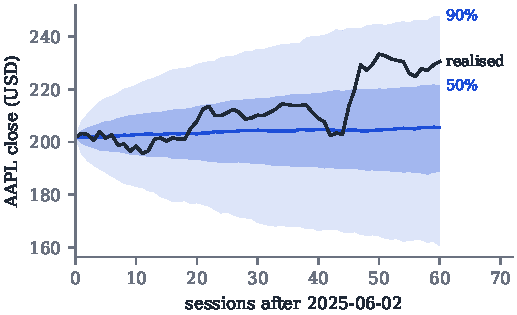
\includegraphics[width=\columnwidth]{fan.pdf}
\caption{2{,}000 sampled AAPL paths from 2 June 2025, inside the test period (shaded: central 50\%
and 90\%), and the path that followed. The fan states width, not direction.}
\label{fig:fan}
\end{figure}

\subsection{Learning from outcomes, weights frozen}
\label{sec:online}
A temperature $T$ rescales the logits $z$. After each realised return it takes one exact gradient
step on the log score,
\begin{equation}
\frac{\partial\,(-\log p_y)}{\partial \log T} = \frac{z_y - \mathbb{E}_p[z]}{T}.
\end{equation}
Replaying the test period day by day, each forecast is scored before its outcome is
learned~\cite{Dawid_1984}. Over 93{,}437 returns this improves the log score by
$0.0078 \pm 0.0017$ nats per return, 4.6 standard errors blocked by month. The frozen model was
already calibrated: its central 90\% interval held 89.9\% of outcomes. $T$ ranged from 0.51 to 2.88.
This is the research question answered on the numeric side: the forecast improves from feedback while
the model under it stays fixed.

\subsection{Serving}
The server draws paths with the generator only while its own artifact records a win over GARCH of
more than one standard error. Otherwise GARCH draws them. Every response carries a sentence stating
that the paths show width, not direction. Synthetic data is written with a sidecar recording the
drawer, the checkpoint digest, the seed and the as-of date.

\section{Challenges and Measurement Traps}
\label{sec:traps}
Each item below produced a wrong conclusion before it was caught.
\begin{enumerate}
\item \textbf{Two numbers, two row sets.} The price head once ``tied'' persistence, 46.9\% against
47.0\%. The head had been scored on the first 1{,}920 windows, which covered 7 of 101 tickers.
\item \textbf{A probe that leaked.} An intent probe scored 90\% on an encoder with no task training,
because a reserved phrasing matched another reserved phrasing.
\item \textbf{Loss picks worse models.} A loss-selected checkpoint generated with 17.2\% unsupported
figures, against 2.4\% for the final one, and 77.0\% exact match against 94.5\%. All promotion now
rests on generation.
\item \textbf{Plateaus that look like limits.} Judged at step 3{,}000, the grounded generator ``could
not copy''. It could by step 4{,}000.
\item \textbf{Noise minima.} Scored on 64 generated answers, one DPO run promoted a checkpoint at 79.5\%
unsupported figures in the sequence 93.3, 90.5, 79.5, 97.9, 100.0.
\item \textbf{The machine slept.} Pretraining launched without a sleep inhibitor logged 15.5\,h of
wall-clock time but only 39\,min of CPU, reaching step 1{,}400 of 49{,}232.
\item \textbf{Serving bugs invisible to tests.} The guard refused grounded answers because decoding
put a space between a minus sign and its digits, reading $-5.6\%$ as $5.6\%$. Every existing test
wrote the sign attached, so the suite was green. Separately, token ids stored as \texttt{uint16}
wrap the $-100$ ignore index to 65{,}436, a valid vocabulary index, unless widened first.
\item \textbf{Reward hacking.} DPO won its objective by writing ``you'' (Section~\ref{sec:preference}).
\item \textbf{Dirty data.} Price files contain returns of 410 scale units and years of zero
movement. Both are rejected loudly rather than repaired.
\item \textbf{Compute.} Everything ran on CPU. The generator trains at about 1.3 steps/s, and one
preference run takes about an hour, so every experiment was budgeted before launch.
\end{enumerate}

\section{Threats to Validity}
The 101 tickers were chosen in 2026, so the price history carries survivorship bias. Nothing here
estimates returns net of transaction costs, and no trading claim is made. Most runs use one seed. The
60-pair label audit and the agent-side feedback labels were written by an AI assistant, not a domain
expert. The feedback logs are small: 118 rows for the abstention curve and 20 turns for the live
session. The return test period (2023 to 2026) is one market regime. Online temperature learning was
run at a single step size.

\section{Conclusion}
A from-scratch agent can learn from feedback without retraining its model. In this system that
learning showed up in three places: a threshold solved from outcomes, a router reading frozen
weights, and a temperature moved by each realised return. Each gain is measured and beats a stated
baseline. Changing the weights from community preferences did not help, and the reason was the data,
not the algorithm: half the corpus states figures its evidence does not contain, and removing
those rows cut answers with an invented figure from 41.0\% to 11.3\%. On prices, the
distribution is learnable and the direction is not. A small tokenised generator beats GARCH-t on the
log score and generates paths with realistic tails and leverage, while its multi-day forecasts only
tie. The most transferable lesson is methodological. Every false conclusion in this project came from
measurement, not modelling, and each was caught by insisting on identical rows, held-out periods and
generate-and-check.

\section*{Acknowledgment}
Development, experiment execution and drafting of this paper were assisted by Claude, an AI assistant
by Anthropic. It also produced the 60-pair label audit and the agent-side feedback labels, as stated
in the text. All numbers come from logged runs in the project repository.

\bibliographystyle{IEEEtran}
\bibliography{refs}

\end{document}
